%%%%%%%%%%%%%%%%%%%%%%%%%%%%%%%%%%%%%%%%%%%%%%%%%%%%%%%%%%%%%%%%%%% 
%                                                                 %
%                            CHAPTER THREE                         %
%                                                                 %
%%%%%%%%%%%%%%%%%%%%%%%%%%%%%%%%%%%%%%%%%%%%%%%%%%%%%%%%%%%%%%%%%%% 
 
\chapter{MATRIX-FREE, INEXACT SOLUTION OF THE LINEAR SYSTEMS}\label{chap:linsys}
During the execution of Algorithm~\ref{alg:pc}, the tangent linear system and
Newton update are solved many times.  Therefore, in order for the
predictor-corrector algorithm to be competitive, these systems must be
(inexactly) solved with high efficiency.  Both systems, \eqref{eq:predictorx}
and \eqref{eq:cor}, take the form
\begin{equation}\label{eq:linsys}
  (\nabla_q H) x = b,
\end{equation}
where $b \in
\mathbb{R}^{N}$ is either $F - G$, in the case \eqref{eq:predictorx} for the tangential step or $-H$ in the case of \eqref{eq:cor} for a Newton step.  We inexactly solve these systems using a preconditioned
Krylov-iterative method.  The primary challenge with this approach, as discussed
in the introduction, is that the preconditioner itself must be matrix free.

In this Chapter, the Krylov iterative solver is briefly reviewed; then the bulk of the content focuses on
the matrix-free preconditioner for the two linear systems. 

\section{Krylov Iterative Solver}
We use the flexible generalized minimal residual method,
FGMRES~\cite{Saad1993fgmres}, to solve~\eqref{eq:linsys}.  One advantage of
FGMRES, compared to most Krylov-based methods, is that is permits nonstationary
preconditioners that vary from one Krylov iteration to the next.  While we do
not take advantage of nonstationary preconditioners in this work, we have found
this flexibility invaluable in the solution of multidisciplinary optimization
problems~\cite{dener:idf2017, dener:2014}.

To find an approximate solution to \eqref{eq:linsys}, FGMRES orthonormalizes a
sequence of matrix-vector products using a generalized form of Arnoldi's
method~\cite{saad:2003}.  Starting with $v_{1} = b/\|b\|$, the generalized
Arnoldi's method produces the following relation at the $i$th iteration:
\begin{equation}\label{eq:arnoldi}
  (\nabla_q H) \mat{Z}_{i} = \mat{V}_{i+1} \bar{\mat{H}}_{i},
\end{equation}
where $\mat{V}_{i+1} \in \mathbb{R}^{N\times (i+1)}$ has orthogonal columns and
$\bar{\mat{H}}_{i} \in \mathbb{R}^{(i+1)\times i}$ is upper Hessenberg.  The
vectors in $\mat{Z}_{i} \in \mathbb{R}^{N\times i}$ form the subspace from which
the approximate solution to \eqref{eq:linsys} is drawn (see below).  These
vectors are related to the vectors in $\mat{V}_{i+1}$ by
\begin{equation*}
  z_{j} = P_j(v_{j}), \qquad \forall j = 1,2,\ldots,i,
\end{equation*}
where $P_j(\cdot)$ denotes the preconditioning operation at iteration $j$.    

The FGMRES solution is given by $x_{i} = \mat{Z}_{i} y_{i}$, where $y_{i}$ is
chosen to minimize the 2-norm of the residual, $r_i \equiv b -  (\nabla_q H) x_i = b -  (\nabla_q H)\mat{Z}_i y_i$, as
follows:
\begin{align*}
  y_{i} = \underset{y \in \mathbb{R}^i}{\textrm{argmin}}
  \lVert b -  (\nabla_q H) \mat{Z}_i y \| 
  &= \underset{y \in \mathbb{R}^i}{\textrm{argmin}}
  \lVert \mat{V}_{i+1} (\|b\| e_1 - \bar{\mat{H}}_{i} y \| \\
  &= \underset{y \in \mathbb{R}^i}{\textrm{argmin}}
  \lVert \|b\| e_1 - \bar{\mat{H}}_{i} y \|,
  \qquad\qquad\text{(since $\mat{V}_{i+1}^T \mat{V}_{i+1} = \mat{I}$)}
\end{align*}
where $e_{1} \in \mathbb{R}^{i+1}$ is the first column of the $(i+1)\times(i+1)$
identity. The minimization problem on the final line is inexpensive to solve in
practice, since $i$ is usually less than 100.

Like most Krylov iterative methods, the FGMRES algorithm described above does
not require the Jacobian $(\nabla_q H)$ explicitly.  From the user's
perspective, the algorithm only requires matrix-vector products and
preconditioning operations.  In this work, matrix-vector products involving
$(\nabla_q H)$ are computed using second-order adjoints~\cite{wang:1992,
  hicken:inexact2014}.  Briefly, each product with $(\nabla_q H)$ requires the
solution of two discretized linear PDEs: a linear forward problem and a linear
adjoint problem.  See \cite{dener:scitech2015} for further details regarding
second-order adjoints in the context of reduced-space problems with state
constraints.  The second required operation, preconditioning, is described in
the next subsection.


\section{Matrix-free Preconditioner}\label{sec:matfreepc}
As $\mu$ approaches zero, the system \eqref{eq:linsys} becomes an increasingly
ill-conditioned saddle-point problem.  Consequently, solving this problem with
an iterative Krylov solver like FGMRES requires an effective preconditioner.  

Many specialized preconditioners have been developed for saddle-point
problems~\cite{benzi2005numerical}, including those arising in full-space
PDE-constrained optimization; see, for example,~\cite{Rees2010optimal}.
However, most full-space PDE-constrained optimization preconditioners rely on
the availability of a matrix-based preconditioner for the state Jacobian. There
is no analogous matrix-based preconditioners for the total Jacobian $\nabla_x g$
in the reduced-space, and, as explained in the introduction, forming $\nabla_x
g$ explicitly is not feasible.  Therefore, one of the primary contributions of
this work is a matrix-free\footnote{In this context, matrix-free means that we
  do not require a matrix whose size is the same size as $\nabla_x g$; however,
  we do use low-rank matrices.} preconditioner for reduced-space PDE-constrained
optimization with state-based constraints.

An effective preconditioner should be inexpensive to apply and approximate the
action of the inverse Jacobian in some sense: $P_j(u) \approx (\nabla_q H)^{-1}
u$ where $u \in \mathbb{R}^{N}$ is arbitrary.  To motivate our preconditioner,
we begin by examining the exact Jacobian $\nabla_q H$ in  \eqref{eq:predictorx} and \eqref{eq:cor}, 
\begin{equation}\label{eq:dHdq}
\begin{aligned}
\nabla_q H &= (1 - \mu) \nabla_{q} F(q) + \mu \nabla_q G(q,q_0) \\
&=  (1-\mu)\begin{bmatrix}
 \nabla_{xx} \mathcal{L}   & \boldsymbol{0} & \mathcal{A}^T_h   & \mathcal{A}^T_g   \\
\boldsymbol{0}     &   - \mat{\Lambda}_g   & \boldsymbol{0} & -\mathcal{S}     \\
\mathcal{A}_h  &  \boldsymbol{0}   & \boldsymbol{0} &  \boldsymbol{0}  \\
\mathcal{A}_g  & -\mathcal{I}  &  \boldsymbol{0}  & \boldsymbol{0}   \\
\end{bmatrix}
+ \mu \begin{bmatrix}
\mathcal{I} & \boldsymbol{0} & \boldsymbol{0} & \boldsymbol{0} \\
\boldsymbol{0}  & \mathcal{I}  & \boldsymbol{0} & \boldsymbol{0} \\
\boldsymbol{0} & \boldsymbol{0} & -\mathcal{I} &  \boldsymbol{0} \\
\boldsymbol{0} & \boldsymbol{0} &   \boldsymbol{0} & -\mathcal{I} 
\end{bmatrix} \\
& = \begin{bmatrix}
	\mat{W}_\mu & \phantom{-}\mat{0} & \phantom{-}\mat{A}_{h,\mu}^T  & \phantom{-}\mat{A}_{g,\mu}^T \\
	\mat{0}  & -\mat{\Lambda}_\mu & \phantom{-}\mat{0}   & -\mat{S}_\mu \\
	\mat{A}_{h, \mu} & \phantom{-}\mat{0} &  -\mu \mat{I} & \phantom{-}\mat{0}  \\
	\mat{A}_{g, \mu} & -(1-\mu)\mat{I} &  \phantom{-}\mat{0}     &   -\mu \mat{I}
\end{bmatrix}
\end{aligned}
\end{equation}
where $\mat{I}$ is the $m\times m$ identity matrix and the sub-Jacobians are
defined by
\begin{gather*}
	\mat{W}_{\mu} \equiv (1-\mu) \left[\nabla_x^2 f + \lambda^T \nabla_x^2 g\right] + \mu \mat{I},\qquad
	\mat{A}_{h, \mu} \equiv (1-\mu) \nabla_x h, \\
	\mat{A}_{g, \mu} \equiv (1-\mu) \nabla_x g, \qquad 
	\mat{S}_{\mu} \equiv (1-\mu)\mat{S},\qquad
	\mat{\Lambda}_\mu \equiv (1-\mu)  \mat{\Lambda}_g - \mu \mat{I}. 
\end{gather*}

In the ideal case, a preconditioner application corresponds to solving the
linear system
\begin{equation}\label{eq:ideal_precond}
  \begin{bmatrix} 
	\mat{W}_\mu & \phantom{-}\mat{0} & \phantom{-}\mat{A}_{h,\mu}^T  & \phantom{-}\mat{A}_{g,\mu}^T \\
	\mat{0}  & -\mat{\Lambda}_\mu & \phantom{-}\mat{0}   & -\mat{S}_\mu \\
	\mat{A}_{h, \mu} & \phantom{-}\mat{0} &  -\mu \mat{I} & \phantom{-}\mat{0}  \\
	\mat{A}_{g, \mu} &  -(1-\mu)\mat{I} &  \phantom{-}\mat{0}     &   -\mu \mat{I}
\end{bmatrix}
\begin{bmatrix} v_x \\ v_s \\ v_{h} \\  v_{g} \end{bmatrix} 
= 
\begin{bmatrix} u_x \\ u_s \\ u_{h} \\ u_{g}  \end{bmatrix},
\end{equation}
where $u_x \in \mathbb{R}^n$, $u_s \in \mathbb{R}^{m}$, and $u_h \in
\mathbb{R}^{l}$,  $u_g \in \mathbb{R}^{m}$.  The following subsections first derive the 
solutions for inequality-only constrained systems, then extend to both equality and inequality 
constrained systems. 

\subsection{Inequality-only Constrained Problems}
When only inequality constraints are present, the linear system \eqref{eq:ideal_precond} 
can be reduced to: 

\begin{equation}\label{eq:ideal_precond_ineq}
  \begin{bmatrix} 
	\mat{W}_\mu & \phantom{-}\mat{0} &  \phantom{-}\mat{A}_{g,\mu}^T \\
	\mat{0}  & -\mat{\Lambda}_\mu & -\mat{S}_\mu \\
	\mat{A}_{g,\mu} &  -(1-\mu)\mat{I} & -\mu \mat{I}
\end{bmatrix}
\begin{bmatrix} v_x \\ v_s \\ v_g \end{bmatrix} 
= 
\begin{bmatrix} u_x \\ u_s \\ u_g \end{bmatrix},
\end{equation}

If at least one constraint is active, it is easy to show that
the lower right $2m \times 2m$ block in the Jacobian will become singular as
$\mu \rightarrow 0$; however, for the moment, we consider the case $\mu > 0$ and
use this block to express $v_s$ and $v_g$ as functions of $v_x$:
\begin{equation}\label{eq:vs_and_vlam}
  \begin{bmatrix} v_s \\ v_g \end{bmatrix}
  =
  \begin{bmatrix}
    \mat{C}_\mu^{-1} & \mat{0} \\
    \mat{0} & \mat{C}_\mu^{-1}
  \end{bmatrix}
  \begin{bmatrix}
    -\mu \mat{I} & \mat{S}_\mu \\
    (1-\mu)\mat{I} & -\mat{\Lambda}_\mu 
  \end{bmatrix}
  \begin{bmatrix} u_s \\ u_g - \mat{A}_{g, \mu} v_x \end{bmatrix},
\end{equation}
where 
\begin{equation*}
  \mat{C}_{\mu} \equiv \mu \mat{\Lambda}_\mu - (1-\mu) \mat{S}_\mu
  = \mu (1-\mu) \mat{\Lambda}_g - \mu^2 \mat{I}- (1-\mu)^2 \mat{S}
\end{equation*}
is a diagonal matrix.  Substituting the expression for $v_g$ from
\eqref{eq:vs_and_vlam} into the first row of \eqref{eq:ideal_precond_ineq}, we find
\begin{equation}\label{eq:schur}
\left[\mat{W}_\mu + \mat{A}_{g, \mu}^T \mat{C}_\mu^{-1} \mat{\Lambda}_\mu \mat{A}_{g,\mu}
  \right] v_x = u_x - \mat{A}_{g,\mu}^T \mat{C}_{\mu}^{-1} \left[(1-\mu) u_s -
  \mat{\Lambda}_\mu u_g \right].
\end{equation}

\begin{remark}
To derive \eqref{eq:vs_and_vlam} and \eqref{eq:schur}, the system matrix in \eqref{eq:ideal_precond_ineq} can be partitioned into a $2 \times 2$ block matrix. 
\begin{equation}\label{eq:sch}
\left[
\begin{array}{c | c c} 
	   \mat{W}_\mu   &   \phantom{-}\mat{0}  &   \phantom{-}\mat{A}_{g,\mu}^T   \\
	   \hline
	   \mat{0}    &   -\mat{\Lambda}_\mu & -\mat{S}_\mu \\
	  \mat{A}_{g,\mu}     &  -(1-\mu)\mat{I} & -\mu \mat{I}   
\end{array}  
\right]
\left[  \begin{array}{c} v_x \\ \hline v_s \\ v_g \end{array} \right]
= 
\left[ \begin{array}{c} u_x \\  \hline u_s \\ u_g \end{array} \right]
\end{equation}
Assuming that $\mat{D}$ is invertible, the solution of the following linear system
\begin{equation*}
\begin{bmatrix}
\mat{A}  & \mat{B} \\
\mat{C}  & \mat{D} 
\end{bmatrix} 
\begin{bmatrix}
x \\ y
\end{bmatrix}
= 
\begin{bmatrix}
a \\ b
\end{bmatrix}
\end{equation*}
can be obtained by: 
\begin{equation}\label{eq:schx}
\begin{aligned}
\left( \mat{A} - \mat{B} \mat{D}^{-1}\mat{C}  \right)x &= a - \mat{B} \mat{D}^{-1}b \\
\mat{C}  x +  \mat{D} y &= b 
\end{aligned}
\end{equation}
Note that the inverse of the lower right block matrix in \eqref{eq:sch} is equivalent to the 
system matrix in \eqref{eq:vs_and_vlam}. 
\begin{equation*}
\begin{bmatrix}
 -\mat{\Lambda}_\mu & -\mat{S}_\mu \\ 
 -(1-\mu)\mat{I} & -\mu \mat{I}  
\end{bmatrix}^{-1} 
= 
\begin{bmatrix}
  \mat{C}_\mu^{-1} & \mat{0} \\
    \mat{0} & \mat{C}_\mu^{-1}
  \end{bmatrix}
  \begin{bmatrix}
   -\mu \mat{I} & \mat{S}_\mu \\
    (1-\mu)\mat{I} & -\mat{\Lambda}_\mu 
  \end{bmatrix}
\end{equation*}
with $\mat{C}_\mu$ being its determinant. Then  \eqref{eq:vs_and_vlam} and 
\eqref{eq:schur} can be derived by filling the corresponding blocks from \eqref{eq:sch} 
to \eqref{eq:schx}.   
\end{remark}

The boundedness of the system \eqref{eq:schur} depends on the behavior of the
matrix $\mat{C}_{\mu}$.  Assuming strict complementarity, as $\mu\rightarrow 0$
we have two situations:
\begin{enumerate}
\item If the constraint is inactive at the solution, then $\lambda_{g,i} = 0$ and
  $\lim_{\mu\rightarrow 0} \left[\mat{C}_\mu^{-1} \mat{\Lambda}_\mu \right]_{ii}
  = 0$.  This has the effective of eliminating the corresponding constraint from
  the reduced system \eqref{eq:schur}.

\item If the constraint is active, then $s_i = 0$ and $\lim_{\mu\rightarrow 0}
  \left[\mat{C}_\mu^{-1} \mat{\Lambda}_\mu \right]_{ii} = \infty$.
\end{enumerate}
The first situation is desirable, since the constraint is inactive and should
not influence the step $v_x$.  The second situation is obviously undesirable;
however, the safeguards in place during the predictor-corrector phases bound the
slacks away from zero, so the inverse of $\mat{C}_{\mu}$ remains well defined in practice.

To cope with the second situation, we use the fraction-to-the-boundary rule 
at the predictor step and the explicit clipping at the end of the corrector step to make sure 
the slack variables are kept away from $\tau_s$ . 
The fraction-to-the-boundary rule we use is slightly 
different than~\cite{Nocedal2006NO} in that we use a fixed absolute value $\tau_s$ as the boundary 
instead of a fixed fraction boundary. 

\begin{remark}
  Consider the case where all the inequality constraints are active.  Then, as
  $\mu\rightarrow 0$, the matrix in \eqref{eq:schur} becomes the Hessian for an
  augmented-Lagrangian-like function with linearized constraints:
  \begin{equation*}
    \lim_{\mu\rightarrow 0} W_{\mu} + \mat{A}_{g,\mu}^T \mat{C}_{\mu}^{-1}
    \mat{\Lambda}_\mu \mat{A}_{g,\mu} = \nabla_x^{2} f + \lambda^T \nabla_x^2 g +
    \frac{1}{\tau_s}\mat{A}_g^{T} \mat{\Lambda}_g \mat{A}_g.
  \end{equation*}
\end{remark}

Having established that \eqref{eq:schur} is well defined for all iterates, we
now seek to approximately invert this system.  To this end, we replace
$\mat{W}_{\mu}$ by an approximation denoted by $\mat{B}_{\mu}$:
\begin{equation*}
\mat{W}_{\mu} \approx \mat{B}_{\mu},
\end{equation*}
where $\mat{B}_{\mu}$ is either a scaled identity, $\mat{B}_{\mu} = \beta
\mat{I}$, or an L-BFGS quasi-Newton approximation~\cite{liu:1989}.  In addition,
we use the Lanczos algorithm~\cite{saad:1992} to construct a low-rank
approximation of $\mat{A}_{g,\mu}^T \mat{C}_\mu^{-1} \mat{\Lambda}_\mu
\mat{A}_{g,\mu}$ for nonlinear constraints; that is
\begin{equation}\label{eq:svd}
  \mat{A}_\mu^T  \mat{C}_\mu^{-1}  \mat{\Lambda}_{\mu}\mat{A}_\mu
  \approx \mat{U} \mat{\Sigma} \mat{V}^T,
\end{equation}
where $\mat{\Sigma} = \textsf{diag}(\sigma_1,\sigma_2,\ldots,\sigma_{\nsig}) \in
\mathbb{R}^{\nsig\times \nsig}$ is a diagonal matrix holding estimates for the
$\nsig$ largest singular values, and $\mat{U} \in \mathbb{R}^{m\times \nsig}$ and
$\mat{V} \in \mathbb{R}^{m\times \nsig}$ are corresponding approximations to the
left and right singular vectors. 

\begin{remark}
  The Lanczos algorithm is advantageous in this context, because it only
  requires matrix-vector products with $\mat{A}_{g,\mu}^T \mat{C}_\mu^{-1}
  \mat{\Lambda}_\mu \mat{A}_{g,\mu}$.  Such products can be evaluated using
  second-order adjoints; again, see \cite{hicken:inexact2014} or
  \cite{dener:scitech2015} for further details regarding second-order adjoints.
  Furthermore, by replacing accurate second-order adjoint PDE solves with
  corresponding preconditioner applications, the cost of the Lanczos-based SVD
  can be significantly reduced.  This idea is explored in the numerical
  experiments.  In our preconditioner, we use a parameter $\mu_e$ 
   to delimit using exact or approximate second-order adjoints. Only after 
   $\mu \leq \mu_e $ the exact second-order adjoints are used in the preconditioner 
   to save computational cost. 
\end{remark}

%\begin{remark}
%  The constraint Jacobian for bound and linear constraints is readily available,
%  so the Lanczos algorithm is not necessary to approximate $\mat{A}_{g,\mu}^T
%  \mat{C}_\mu^{-1} \mat{\Lambda}_{\mu}\mat{A}_{g,\mu}$ in this case.
%  \todo[inline]{But the matrix $\mat{A}_\mu^T \tilde{\mat{C}}_\mu^{-1}
%    \mat{\Lambda}^{-1}\mat{A}_\mu$ involves products between the nonlinear and
%    linear constraints; how do you account for this in Lanczos?  
%   \padd{ By zeroing the corresponding portions in the middle term  $C_{\mu}*\Lambda$, 
%   the products AXA would be only for the nonlinear constraint part.   The bound constraint
%   part of AXA, which is $C_{\mu}*\Lambda$ times Identity matrix, is added to the Hessian
%   W part.  $B_{\mu}$ is the sum of the Hessian and bound constraint. 
%     }}
%\end{remark}

\begin{remark}
 At the beginning of the homotopy iterations when the activeness of the constraints are far from 
determined, it happens sometimes that  $ \mat{C}_\mu^{-1}  \mat{\Lambda}_{\mu}$ are close to 
vector of zeros, resulting in rank dependent matrix-vector products in Lanczos iterations. To deal 
with this issue, at the beginning, we use $  \mat{A}_\mu^T \mat{A}_\mu
  \approx \mat{U} \mat{\Sigma} \mat{V}^T $ in the preconditioner at the beginning of the homotopy iteration. 
  When $\mu$ gets smaller than $\Sigma_e$, we use \eqref{eq:svd} in the preconditioner. 	
\end{remark}

Using the above approximations, the (approximate) inverse of the matrix in
\eqref{eq:schur} can be found using the Sherman-Morrison-Woodbury formula:
\begin{align}
\left[\mat{W}_\mu + \mat{A}_\mu^T \mat{C}_\mu^{-1}  \mat{\Lambda}_\mu  \mat{A}_\mu \right]^{-1}
&\approx
\left[\mat{B}_{\mu} + \mat{U} \mat{\Sigma} \mat{V}^T \right]^{-1} \notag \\
&= \mat{B}_\mu^{-1} - \mat{B}_\mu^{-1} \mat{U}  \left(  \mat{I}_{\nsig} +  \mat{\Sigma} \mat{V}^{T} \mat{B}_\mu^{-1} 
\mat{U} \right)^{-1} \mat{\Sigma} \mat{V}^{T} \mat{B}_\mu^{-1}.
\label{eq:smw}
\end{align}
where $\mat{B}_\mu^{-1}$ is either $(1/\beta)\mat{I}$ or the L-BFGS
approximation.  Note that, in the above expression, $\left(\mat{I}_{\nsig} +
\mat{\Sigma} \mat{V}^{T} \mat{B}_{\mu}^{-1} \mat{U} \right)$ is an $\nsig\times
\nsig$ matrix.  In the proposed preconditioner, we assume that the number of
singular values in the truncated SVD, \ie $\nsig$, is sufficiently small that we
can invert this matrix explicitly using an $LU$ factorization.

In summary, to approximately solve \eqref{eq:schur} we evaluate
\begin{equation}\label{eq:vx}
  v_x = \left[\mat{B}_\mu^{-1} - \mat{B}_\mu^{-1} \mat{U}  \left(  \mat{I}_{\nsig} +  \mat{\Sigma} \mat{V}^{T} 
  \mat{B}_\mu^{-1} \mat{U} \right)^{-1} \mat{\Sigma} \mat{V}^{T} \mat{B}_\mu^{-1} \right]
  \left\{ u_x - \mat{A}_\mu^T \mat{C}_{\mu}^{-1} \left[(1-\mu) u_s -
  \mat{\Lambda}_\mu u_g \right]\right\}.
\end{equation}

%Note that, in addition to using the approximate inverse \eqref{eq:smw}, we have
%replaced $\mat{C}_{\mu}$ with $\tilde{\mat{C}}_\mu$ on the right hand side.

After obtaining $v_x$, we use it in \eqref{eq:vs_and_vlam} to
find $v_s$ and $v_\lambda$;
\begin{align}
  v_s &= \mat{C}_\mu^{-1}\left[-\mu u_s + \mat{S}_\mu \left( u_g - \mat{A}_\mu v_x\right) \right], \label{eq:vs} \\
  v_\lambda &= \mat{C}_\mu^{-1}\left[(1-\mu)u_s - \mat{\Lambda}_\mu \left( u_\lambda - \mat{A}_\mu v_x \right) \right]. 
  \label{eq:vlam}
\end{align}

\comment{
Note the use of $\mat{C}_\mu^{-1}$ in the first equation and the use of
$\tilde{C}_\mu^{-1}$ in the second equation.  For the first equation,
$\lim_{\mu\rightarrow 0} \mat{C}_\mu = -\mat{S}$, so
\begin{equation*}
  \lim_{\mu\rightarrow 0} v_s = 
  \lim_{\mu\rightarrow 0} \mat{C}_\mu^{-1}\left[-\mu u_s + \mat{S}_\mu \left( u_\lambda - \mat{A}_\mu v_x\right) \right]
  = \mat{A} v_x - u_\lambda,
\end{equation*}
which is consistent with the equation $\mat{A} v_x - v_s = u_\lambda$ that we
obtain from \eqref{eq:ideal_precond}.  In contrast, the update for $v_\lambda$
would be unbounded for active constraints if $\mat{C}_\mu$ were used.
}

We conclude this section by summarizing the complete matrix-free preconditioner
in Algorithm~\ref{alg:precond}.  Note that the approximate SVD can be performed
before each Krylov iterative solve, or it can be performed periodically to
reduce cost, possibly at the risk of descreasing the effectiveness of the
preconditioner.

\LinesNumberedHidden
\begin{algorithm}[tbp]\setstretch{1.35}
\SetKwInOut{Input}{Input}
\SetKwInOut{Output}{Output}
\SetKwInOut{Parameter}{Parameters}
\SetKw{Return}{return}
\SetEndCharOfAlgoLine{}

\Parameter{$c_{\min}$, $\nsig$, and values at which to evaluate matrices, $x$, $s$,
  $\lambda$, and $\mu$}
\Input{vectors to precondition, $u_x$, $u_s$, $u_\lambda$}
\Output{preconditioned vectors, $v_x$, $v_s$, $v_\lambda$}
\BlankLine
Build the truncated and approximate SVD \eqref{eq:svd}, possibly using preconditioner
applications in place of exact second-order adjoint solves \\
Solve for $v_x$ using \eqref{eq:vx}\\
Solve for $v_s$ using \eqref{eq:vs}\\
Solve for $v_\lambda$ using \eqref{eq:vlam}\\
\Return $v_x$, $v_s$, and $v_\lambda$
\caption{Matrix-free, approximate SVD preconditioner. \label{alg:precond}}
\end{algorithm}

\subsection{Both Inequality and Equality Constrained Problems}
When both the equality and inequality constraints are present, it is not obvious to reduce the system in 
\eqref{eq:ideal_precond} using the Schur complement method. However, by using a basic row block by 
row block variable elimination method, a similar reduced system like \eqref{eq:schur} can be obtained. 
\begin{equation}\label{eq:2}
  \begin{bmatrix} 
	\mat{W}_\mu & \phantom{-}\mat{0} & \phantom{-}\mat{A}_{h,\mu}^T  & \phantom{-}\mat{A}_{g,\mu}^T \\
	\mat{0}  & -\mat{\Lambda}_\mu & \phantom{-}\mat{0}   & -\mat{S}_\mu \\
	\mat{A}_{h, \mu} & \phantom{-}\mat{0} &  -\mu \mat{I} & \phantom{-}\mat{0}  \\
	\mat{A}_{g, \mu} &  -(1-\mu)\mat{I} &  \phantom{-}\mat{0}     &   -\mu \mat{I}
\end{bmatrix}
\begin{bmatrix} v_x \\ v_s \\ v_{h} \\  v_{g} \end{bmatrix} 
= 
\begin{bmatrix} u_x \\ u_s \\ u_{h} \\ u_{g}  \end{bmatrix},
\end{equation}
The slack variable $v_s$ can be represented by the inequality multipliers $v_g$ using 
the second row block of \eqref{eq:2}: 
% \begin{equation}
\begin{align}
 -\mat{\Lambda}_\mu  v_s  - \mat{S}_\mu v_g  &= u_s  \notag \\
   -v_s &=   \mat{\Lambda}_\mu ^{-1} \left[ \mat{S}_\mu v_g + u_s  \right]  
 \label{eq:vs2}
\end{align}
% \end{equation}
By plugging \eqref{eq:vs2} into the last row block of \eqref{eq:2}, the inequality multiplier $v_g$ is 
left to be represented by $v_x$ only: 
  %\label{eq:vg}
\begin{align}
\mat{A}_{g,\mu} v_x -(1-\mu)\mat{I} v_s -\mu \mat{I} v_g  &= u_g  \notag \\
\mat{A}_{g,\mu} v_x   +  (1-\mu)   \mat{\Lambda}_\mu ^{-1} \left[ \mat{S}_\mu v_g + u_s  \right] -\mu \mat{I} v_g &= u_g  \notag  \\
 v_g = \left[ (1-\mu)   \mat{\Lambda}_\mu ^{-1} \mat{S}_\mu   -\mu \mat{I} \right]^{-1} & \left[   u_g -    (1-\mu)   \mat{\Lambda}_\mu ^{-1} u_s  -   \mat{A}_{g,\mu} v_x   \right] 
 \label{eq:vg2x}
\end{align}
The first row block of \eqref{eq:2} can be rewritten using $v_g$ as in \eqref{eq:vg2x}:
\begin{equation*}
 \mat{W}_\mu v_x +  \mat{A}_{h,\mu}^T v_h  + \mat{A}_{g,\mu}^T  \left[ (1-\mu)   \mat{\Lambda}_\mu ^{-1} \mat{S}_\mu   -\mu \mat{I} \right]^{-1} \left[  u_g -    (1-\mu) \mat{\Lambda}_\mu ^{-1} u_s  -   \mat{A}_{g,\mu} v_x   \right] =u_x 
 \end{equation*}
\begin{equation*} 
\begin{aligned}
\left[ \mat{W}_\mu +  \mat{A}_{g,\mu}^T \left[ (1-\mu) \mat{\Lambda}_\mu ^{-1} \mat{S}_\mu   -\mu \mat{I} \right]^{-1} (-\mat{A}_{g,\mu})  \right]v_x  +  \mat{A}_{h,\mu}^T v_h &= \\
u_x - \mat{A}_{g,\mu}^T \left[ (1-\mu)  \mat{\Lambda}_\mu ^{-1} \mat{S}_\mu   -\mu \mat{I} \right]^{-1}  &\left[ u_g -   (1-\mu)  \mat{\Lambda}_\mu ^{-1} u_s  \right] 
\end{aligned}
\end{equation*}
The reduced system becomes: 
\begin{multline}\label{eq:schur_equ}
\begin{bmatrix}
\mat{W}_\mu +  \mat{A}_{g,\mu}^T \left[(1-\mu)  \mat{\Lambda}_\mu ^{-1} \mat{S}_\mu   -\mu \mat{I} \right]^{-1} (-\mat{A}_{g,\mu})    & \phantom{-}\mat{A}_{h,\mu}^T   \\
\phantom{-}\mat{A}_{h,\mu}  & \phantom{-}-\mu \mat{I}
\end{bmatrix}
\begin{bmatrix} v_x \\ v_h  \end{bmatrix} 
= \\
\begin{bmatrix} u_x - \mat{A}_{g,\mu}^T \left[ (1-\mu)  \mat{\Lambda}_\mu ^{-1} \mat{S}_\mu   -\mu \mat{I} \right]^{-1} \left[ u_g -    (1-\mu)  \mat{\Lambda}_\mu ^{-1} u_s  \right] \\ u_h  \end{bmatrix} 
\end{multline}
Now pay attention that in $\mat{C}_\mu^{-1} \mat{\Lambda}_\mu $ in  \ref{eq:schur} is equivalent to : 
\begin{equation*}
\begin{aligned}
\mat{C}_\mu^{-1} \mat{\Lambda}_\mu &=\left[ \mu \mat{\Lambda}_\mu - (1-\mu) \mat{S}_\mu \right]^{-1}  \mat{\Lambda}_\mu \\
	&=  \left[ \mu \mat{I} -   (1-\mu) \mat{S}_\mu \mat{\Lambda}_\mu^{-1} \right]^{-1}
\end{aligned}
\end{equation*}
Then \eqref{eq:schur_equ} is equivalent to: 
\begin{equation}\label{eq:schur_equ2}
\begin{bmatrix}
\mat{W}_\mu +  \mat{A}_{g,\mu}^T  \mat{C}_\mu^{-1} \mat{\Lambda}_\mu    \mat{A}_{g,\mu}    & \mat{A}_{h,\mu}^T   \\
\mat{A}_{h,\mu}  & -\mu \mat{I}
\end{bmatrix}
\begin{bmatrix} v_x \\ v_h  \end{bmatrix} 
=
\begin{bmatrix} u_x - \mat{A}_{g,\mu}^T \mat{C}_\mu^{-1}  \left[(1-\mu) u_s  - \mat{\Lambda}_\mu u_g     \right]  \\ u_h  \end{bmatrix} 
\end{equation}
Therefore, when both equality and inequality constraints present, we need to solve \eqref{eq:schur_equ2}, then 
$v_s$ and $v_g$ can be recovered by \eqref{eq:vs_and_vlam} the same way as in inequality-only case.
The focus is how to solve the following system using matrix-free methods: 
\begin{equation}\label{eq:reduce}
\begin{bmatrix}
\mat{W}_\mu +  \mat{A}_{g,\mu}^T  \mat{C}_\mu^{-1} \mat{\Lambda}_\mu  \mat{A}_{g,\mu}    & \mat{A}_{h,\mu}^T   \\
\mat{A}_{h,\mu}  & -\mu \mat{I}
\end{bmatrix}
\begin{bmatrix} v_x \\ v_h  \end{bmatrix} 
=
\begin{bmatrix} \text{rhs}   \\ u_h  \end{bmatrix} 
\end{equation}
Note that the first row block in the right-hand-side of \eqref{eq:schur_equ2} is denoted by $\text{rhs}$ in \eqref{eq:reduce}.  
Once again we draw our insights from the Schur complement equation. 
\begin{remark}
Assuming that $\mat{D}$ is invertible, the solution of the following linear system 
\begin{equation*}
\begin{bmatrix}
\mat{A}  & \mat{B} \\
\mat{C}  & \mat{D} 
\end{bmatrix} 
\begin{bmatrix}
x \\ y
\end{bmatrix}
= 
\begin{bmatrix}
a \\ b
\end{bmatrix}
\end{equation*}
can be obtained by, 
\begin{equation*}
\begin{bmatrix}
x \\ y
\end{bmatrix}=
\begin{bmatrix}
\mat{A}  & \mat{B} \\
\mat{C}  & \mat{D} 
\end{bmatrix} ^{-1}
\begin{bmatrix}
a \\ b
\end{bmatrix}
\end{equation*}
where 
\begin{equation}\label{eq:schur_inv}
\begin{bmatrix}
A & B \\ C & D 
\end{bmatrix} ^{-1}
= \begin{bmatrix}
I  & 0 \\
-D^{-1}C  & I 
\end{bmatrix}
 \begin{bmatrix}
( A-BD^{-1}C )^{-1}   &  0 \\
 0   & D^{-1} 
\end{bmatrix}
\begin{bmatrix}
I  &   -BD^{-1} \\
0  &  I 
\end{bmatrix}
\end{equation}
\end{remark}
To apply the Schur complement inverse to \eqref{eq:reduce}, we have to consider two situations: 
\begin{enumerate}
\item When $\mu$ is not so small, e.g. $\mu > \tau_{\mu}$ then $- \mu \mat{I}$ is invertible and we can use \eqref{eq:schur_inv}. 
\item When $\mu$ gets close to zero, e.g. $\mu < \tau_{\mu}$, we enforce the following clipping rule $\mu = \max(\mu, \tau_{\mu}) $ 
to prevent $\mu$ from being too small in the preconditioner, where we use $\tau_{\mu} = 10^{-4}$ in the numerical experiments. This way \eqref{eq:schur_inv} can still be used.
\end{enumerate}
This way, $v_x$ and $v_h$ can be solved by: 
\begin{equation}\label{eq:core_equ}
\begin{bmatrix} v_x \\ v_h  \end{bmatrix} 
=
\begin{bmatrix}
I & 0 \\
\frac{1}{\mu} \mat{A}_{h,\mu}  &  I 
\end{bmatrix}
\begin{bmatrix}
\left(\mat{W}_\mu +  \mat{A}_{g,\mu}^T  \mat{C}_\mu^{-1} \mat{\Lambda}_\mu  \mat{A}_{g,\mu}  
+ \frac{1}{\mu}  \mat{A}_{h,\mu}^T \mat{A}_{h,\mu} \right)^{-1}    & 0 \\
0  &  -\frac{1}{\mu}\mat{I} 
\end{bmatrix}
\begin{bmatrix}
I  & \frac{1}{\mu} \mat{A}_{h,\mu}^T  \\
0  &  I
\end{bmatrix}
\begin{bmatrix}
rhs  \\ u_h
\end{bmatrix}
\end{equation}
where the major component is the following operation besides the matrix-vector product operations with $\mat{A}_{h,\mu}$: 
\begin{equation}
\left(\mat{W}_\mu +  \mat{A}_{g,\mu}^T  \mat{C}_\mu^{-1} \mat{\Lambda}_\mu  \mat{A}_{g,\mu}  
+ \frac{1}{\mu}  \mat{A}_{h,\mu}^T \mat{A}_{h,\mu} \right)^{-1}  y
\end{equation}
where $y$ refers to 
\begin{equation}
y = \text{rhs} + \frac{1}{\mu} \mat{A}_{h,\mu}^T u_h
\end{equation}
By stacking $ \mat{A}_{h,\mu} $ and $\mat{A}_{g,\mu}$ together, 
the following expressions can be derived: 
\begin{equation}
\mat{W}_\mu  +  \mat{A}_\mu ^T \Sigma_{\mu} \mat{A}_\mu = 
\mat{W}_\mu +  \mat{A}_{g,\mu}^T  \mat{C}_\mu^{-1} \mat{\Lambda}_\mu  \mat{A}_{g,\mu}  
+ \frac{1}{\mu}  \mat{A}_{h,\mu}^T \mat{A}_{h,\mu} 
\end{equation}
where 
\begin{equation}
\begin{aligned}
 \mat{A}_\mu &= 
 \begin{bmatrix}
 \mat{A}_{h,\mu} \\
 \mat{A}_{g,\mu}
 \end{bmatrix} \\
  \Sigma_{\mu} &= 
  \begin{bmatrix}  
  \frac{1}{\mu} \mat{I}  & 0 \\
  0   &  \mat{C}_\mu^{-1} \mat{\Lambda}_\mu 
  \end{bmatrix}
 \end{aligned}
\end{equation}
This way we can use Sherman-Morrison to compute the inverse of 
$\mat{W}_\mu  +  \mat{A}_\mu ^T \Sigma_{\mu} \mat{A}_\mu$, and use Lanczos method to find the SVD 
approximation of $\mat{A}_\mu ^T \Sigma_{\mu} \mat{A}_\mu$, in the same manner as in the previous section. 

\section{Application: Scalable Quadratic Optimization Problem}
\subsection{Problem Description}
The next numerical experiement is intended to test the effectiveness of the approximate SVD
preconditioner defined in Algorithm~\ref{alg:precond}.  In particular, we are
interested in the performance of the algorithm with the preconditioner as the size of the problem increases.  
To this end, we consider the following scalable optimization problem
in which we can independently control the size and conditioning of the Hessian
and constraint Jacobian:
\begin{equation}\label{eq:quadra}
  \begin{aligned}
    &\underset{x \in R^n} {\text{min}}  
    & & \frac{1}{2}x^T \mat{Q} x + g^T x \\
    &\text{subject to} & & \mat{A}x \geq b  \\
  \end{aligned}.
\end{equation}
The vectors $g\in \mathbb{R}^{n}$ are randomly sampled from a uniform distribution 
in $[ 0,1)$, while $b \in \mathbb{R}^{n}$ from $[0,0.1)$. 

The Hessian $\mat{Q}$ is diagonal with entries
\begin{equation*}
  \mat{Q}_{ii} = \begin{cases}
    \frac{1}{i}, &  i = 1, 2, ...,  \kappa, \\
    \frac{1}{\kappa}, & i =  \kappa+1, ... , n, \\
  \end{cases}
\end{equation*}
where $\kappa \leq n$.  This definition produces a Hessian with a condition
number of $\kappa$,  so that the condition number
stays the same as the dimension of the problem increases from $100$ to $500$. 

The constraint Jacobian $\mat{A} \in \mathbb{R}^{n\times n}$ is defined as follows. Suppose
$\mat{D} \in \mathbb{R}^{n\times n}$ is a diagonal
matrix of singular values defined similar to $\mat{Q}$:
\begin{equation*}
  \mat{D}_{ii} = \begin{cases}
    \frac{1}{i^2}, &  i = 1,2,...,\nu, \\
    \frac{1}{\nu^2}, & i = \nu+1, ..., n, \\
  \end{cases}
\end{equation*}
where $\nu \leq n$.  Then, $\mat{A}_L $ and $\mat{A}_R$ are matrices of random integers from 
the discrete uniform distribution in the
interval [0,10),  which are applied with $QR$ factorizations,  
\begin{equation*}
\begin{aligned}
\mat{A}_L &= \mat{Q}_L \mat{R}_L \\
\mat{A}_R &= \mat{Q}_R \mat{R}_R \\
\end{aligned}
\end{equation*}
The constraint Jacobian $\mat{A} =\mat{Q}_L  \mat{D} \mat{Q}_R $ 

Consequently, the condition number of $\mat{A}$ is also constant $\nu ^2$ when the dimension 
of the problem increases. 


For this study we chose $\kappa = \nu = 9$, which gives the condition number 
$ \text{cond} (\mat{Q} )= 9$,  $ \text{cond} (\mat{A}) = 81$. The modest condition number of 
$\mat{Q} $ and $\mat{A}$ is benefit to our study in that we can shift 
the focus to treat the ill-condition in the KKT matrix 
$\nabla_{q} F(q)$ at $\mu<\epsilon_{\mu}$, whose typical condition number ranges from $10^4$ to $10^9$
depends on the problem.

The values of $\kappa$ and $\nu$ are chosen to be a fixed positive
value smaller than the number of design variables.  This is to make the
condition number of the matrix fixed, not hugely increasing with the
dimension of the problem.

\begin{remark}
Although the matrices for this synthetic problem are available explicitly, our
algorithm does not exploit this and remains matrix-free, \ie it only uses
matrix-vector products.
\end{remark}

\subsection{Results}
Figure~\ref{fig:quad_hist} plots the absolute optimality, complementarity and feasibility
histories versus CPU time. 
The predictor-corrector algorithm is applied both with and without the preconditioner.  
In addition, the plots include the results
from SNOPT~\cite{gill:2002}, a well-validated active-set SQP
optimization library.

Without the preconditioner, the predictor-corrector algorithm is not competitive
and does not converge after sufficient time.  This illustrates the need for preconditioning Newton-Krylov
optmization algorithms, even for modest sized problems.  The results
also indicate that the proposed algorithm outperforms SNOPT on this particular
problem.  SNOPT is able to establish feasiblity within the same time as the
predictor-corrector algorithm, but it takes significantly longer to converge the
first-order optimality conditions.

\begin{figure}[tbp]
  \centering
  \subfloat[$n=200$\label{fig:quad_200}]{
   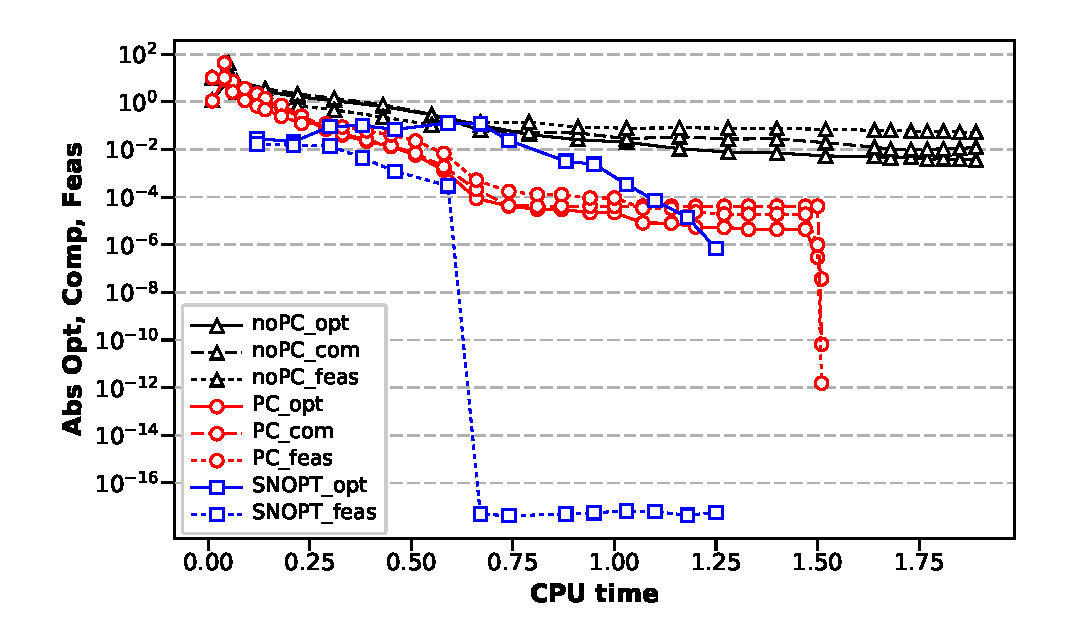
\includegraphics[clip,width=0.7\linewidth]{./figs/chap4_test/quadratic_200_color.eps} }
   \hspace{1em}
   \subfloat[$n=500$\label{fig:quad_500}]{
   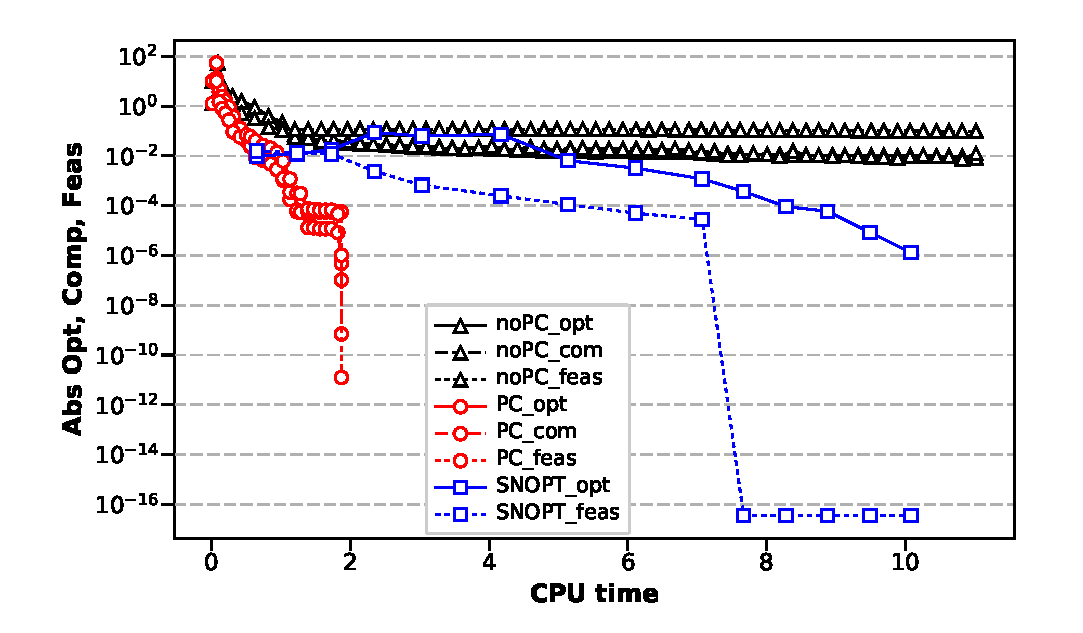
\includegraphics[clip,width=0.7\linewidth]{./figs/chap4_test/quadratic_500_color.eps} }
   \caption{Convergence histories for the quadratic problem with $n=200$ and
  $n=500$. The results for the proposed algorithm, with and without
  preconditioning, are plotted together with the results from
  SNOPT.\label{fig:quad_hist}}
\end{figure}

To further explore the scalability of the proposed algorithm, we run 100 random cases for 
each fixed sized problem, for $n = 100, 200, 300, 400, 500$.  In each random case, the gradient 
in the objective function $g$, and the right hand side vector $b$ in the linear constraint in \eqref{eq:quadra} 
are randomly generated. The diagonal Hessian $\mat{Q}$ and $\mat{D}$ is fixed, while $\mat{A}_L$ and $\mat{A}_R$ are randomly generated. So the constraint Jacobian $\mat{A}$ is also changing. The starting point for each run is also randomly generated. Figure~\ref{fig:quad_scale} shows the error bar of the CPU time while
the problem size increases. As can be seen, the new method exhibits good scalability performances, in comparison with SNOPT. 

\begin{figure}[tbp]
  \centering
  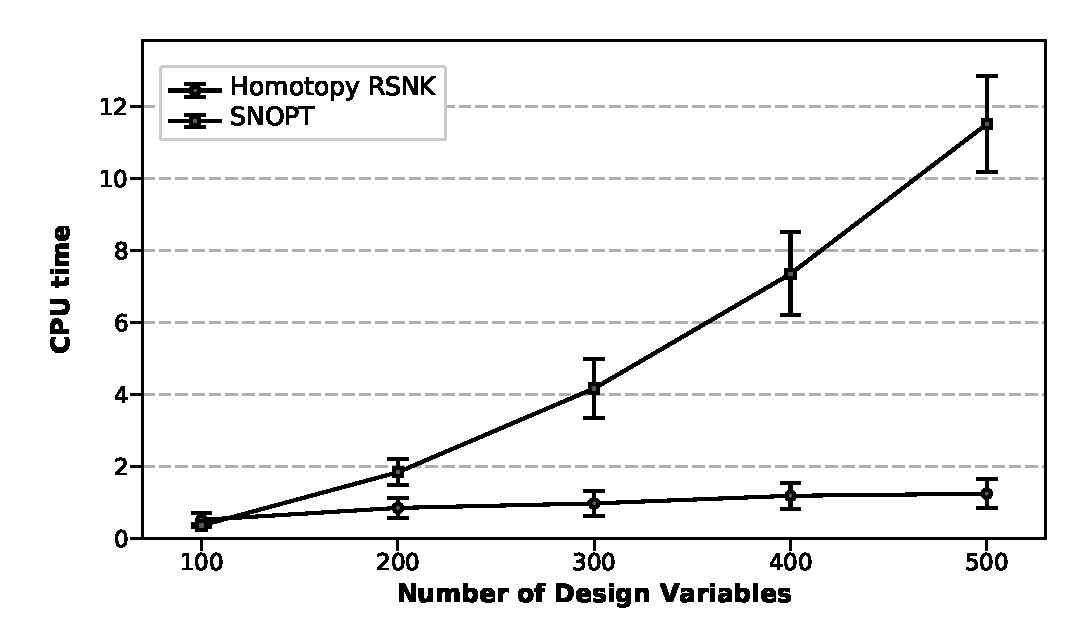
\includegraphics[clip,width=0.8\textwidth]{./figs/chap4_test/quadratic_random_100_nocolor.eps}%
  \caption{CPU cost versus number of design variables for the quadratic
    optimization problem.\label{fig:quad_scale}}
\end{figure}

It is worthwhile to emphasize that the proposed SVD preconditioner is particularly effective for this constructed problem, because the problem is designed in such a way that the distribution of the singular values for the constraint Jacobian is readily separable, with the largest few dominates, and there are only linear inequality constraints. Put another way, SVD approximation can capture the main characteristics of the matrix in~\eqref{eq:svd}. For real-world problems, the distribution of the singular values of the constraint Jacobian is unknown, and may possess unfavorable distribution patterns. The the proposed preconditioner may not be as effective.  






